%WP7 Fred
%URL for CTT - short!!!!
%Coquand et al. Ghani, Neil Ghani, %Spell, fullsptop
%TXA M$
%check leadership and seconds, esp WP4,5
%choice of collabs - went for the best.
%We do impact
%This project treads a
%fine balance between being well scoped so that we can achieve theirs
%goals within the allocated period of study while simultaneously being
%ambitious enough to have a major and lasting impact upon how we
%compute.  
%First safety critical, then more generally ...
%Say we dont do Agda scale systems so Power-esque quotes possible.
%TIC
%Changyu
%Already HoTT is impacting Coq

%cross documents
%============
%Unify JoR, WPs and TRs and unify citations, eg TXA M$

%checks
%====
%letters, quotes


%Why no one else (JoR)
%Indivdual small steps are being taken
%==========
%Developed by mathematicians
%rebuilding it - our track record of converting maths to PL
%Why has no one done it before. Have we balls or insight



%Humility
%========
%In risk ok .. too much, too little? Feasability. Structured with
%What we dont claim. Power ...
%Srtength:transforms, contributes, feeds into etc.
%No overstretch (POC)
%Dissing others (AS + PW). We are formal methods (GC)
%WP7 is still POC.
%acheivable POCS for overall ambitious result with individual ambition too.
%All WPS are POCs for our technology.
%generate impact or pathways to generate impact. open to door?
%potential demonstrayted vs results achieved
%proper argument for transforming the foundation of PL/PV. 
%Homoptical foundations for PLPV







\documentclass[a4paper,11pt]{article}

\usepackage[top=2cm, bottom=2cm, left=2cm, right=2cm]{geometry}

\usepackage{mathptmx}
\usepackage{epsf}           %\input{epsf}
\usepackage{amsfonts}
\usepackage{amstext}
\usepackage{amssymb}
\usepackage{url}
%\usepackage[dvips]{graphics}
\usepackage[dvips,pdftex]{graphicx}
\usepackage[dvips,all]{xy}
\usepackage{multicol}
\usepackage{natbib}
\setlength{\bibsep}{0.0pt}

\usepackage{microtype}

\usepackage{hyperref}

%\newlength{\extraplusheight}
%\newlength{\extrapluswidth}
%\setlength{\extraplusheight}{4.7cm}
%\setlength{\extrapluswidth}{4.7cm}
%\addtolength{\textwidth}{\extrapluswidth}
%\addtolength{\textheight}{\extraplusheight}
%\addtolength{\oddsidemargin}{-.5\extrapluswidth}
%\addtolength{\evensidemargin}{-.5\extrapluswidth}
%\addtolength{\topmargin}{-0.5\extraplusheight}
\setlength{\parindent}{0 pt}
\setlength{\parskip}{.5ex}

\newcommand{\eg}{{e.g.}\ }

\newcommand{\Int}[1]{[\![ #1 ]\!]}
\newcommand{\malign}[1]{\begin{array}[t]{@{}l@{\;}l@{}l@{}} #1 \end{array}}
\newcommand{\logrel}[2]{\Delta_{#1,#2}}
\newsavebox{\fminibox}
\newenvironment{fminipage}
 {\begin{lrbox}{\fminibox}\begin{minipage}{8cm}\vspace*{-2ex}}
 {\\[-2ex]\vspace*{-2ex}\end{minipage}\end{lrbox}\noindent\centerline{\fbox{\usebox{\fminibox}}}\vspace{0.5ex}}   

%\setlength{\parindent}{0.15in}
%\setlength{\parskip}{0.3ex}

% Discourage unnecessary hyphenation.
\sloppy\hyphenpenalty 4000

\newcommand{\ra}{\rightarrow}
\newcommand{\A}{\mathcal{A}}
\newcommand{\E}{\mathcal{E}}
\newcommand{\C}{\mathcal{C}}
\newcommand{\B}{\mathcal{B}}
\newcommand{\Set}{\mbox{{\sf Set}}}
\newcommand{\Nat}{\mathit{Nat}}
\newcommand{\Alge}[1]{\mathit{Alg}_{#1}}
\newcommand{\hash}{\#}

\begin{document}

\thispagestyle{plain}
\begin{center}
  {\Large {\bf Homotopy Type Theory: Programming and Verification}}\\[1ex] 
\vspace*{-0.1in}

%  {\Large \bf Case for Support}\\[1ex]
  \rule{140mm}{.5mm}\\[2ex]
\end{center}

\noindent
{\bf \Large Part 1A: Previous Research \& Track Record}

\textbf{Professor Neil Ghani.} Neil Ghani was appointed to a
Professorship in 2008 at the University of Strathclyde, where he
founded the Mathematically Structured Programming (MSP) group. His
research on a number of topics feeds directly into this the proposal,
\eg i) his work on logical relations~\cite{neil2014relParamDep} feeds
into the development of semantic and syntactic presentations of
Homotopy Type Theory (HoTT) in WP1,2; ii) his work on data types
(containers~\cite{alti:cont-tcs}, quotient
containers~\cite{alti:mpc04}, indexed
containers~\cite{altenkirchGhaniHancockMcBrideMorris:indexedContainers}
and induction-recursion~\cite{ghani:fibredIR}) feed into the
development of higher inductive types in WP3; iii) his work on the
semantics of effects~\cite{atkeyGhaniJacobsJohann:effects} feeds into
the application of HoTT to effects in WP4; iv) his work on
induction-recursion~\cite{ghani:fibredIR} also feeds into the
formalisation of the syntax of HoTT in WP5; and v) his work on Units
of Measure~\cite{uom} (via an Impact Accelerator Account grant held in
collaboration with Microsoft) feeds into HoTT-based computing with
algebraically indexed types in WP8. More generally, Neil Ghani is a
world expert on using semantic structures to drive the development of
type theory and programming languages, exactly the methodology to be
followed in this proposal.

Professor Ghani has attracted \pounds 1.7M in research funding,
comprising \pounds 1.3M as PI on 8 grants and \pounds 400K as CoI in 2
grants.  Indeed, results obtained during his following EPSRC grants
feed directly into this proposal: Theory And Applications of Induction
Recursion (EP/G03298X/1), Reusability and Dependent Types
(EP/G034109/1), Logical Relations for Program Verification
(EP/K023837/1), and Theory and Applications of Containers
(EP/C511964/2). The first two of these were 3-site grants similar in
nature to this proposal and their success demonstrates Ghani's track
record in successfully managing distributed grants of this size. More
generally, Ghani has successfully supervised five PhD students, is
supervising three more, and has supervised four RAs. He organises the
ScotCats seminar series, organised a meeting on HoTT in Ljubljana in
2012, and will host the next UK HoTT meeting in January 2015. He is a
member of the EPSRC Peer Review College and is a SICSA theme leader in
Complex Systems Engineering. Finally, his Impact Accelerator Account
demonstrates a track record of striving to generate impact from EPSRC
funded research --- see {\em Pathways to Impact} for details.

For further information, see~\url{http://cis.strath.ac.uk/~ng}.

\textbf{Dr Conor McBride.} Conor McBride received his PhD from the
University of Edinburgh in 1999 for his work on dependently typed
programming. After this, he worked as an RA at the Universities of
Durham and Nottingham before becoming a lecturer at the University of
Strathclyde in 2008. His work on the foundations and implementations
of non-dependently and dependently typed
programming~\cite{viewftl,alti:ott-conf,easy,mcbride:outrageous} has
become seminal, both via his own programming language Epigram and via
his work with the Agda, Coq, and Haskell teams. He is now widely
regarded as a leader of his field as illustrated by his widely cited
papers (\eg ~\cite{viewftl} has been cited 320 times) and invitations
to keynote addresses at conferences. His work on Observational Type
Theory (a proof irrelevant form of HoTT)~\cite{alti:ott-conf} feeds directly
into WP2, his work on containers~\cite{alti:mpc04} feeds directly into WP3, his
work on effects~\cite{conor:frank} feeds directly into WP4, and his work on
dependently typed programming and formalising the syntax of type
theory in itself~\cite{viewftl,alti:ott-conf,easy,mcbride:outrageous}
feeds directly into WP5--8.

Dr McBride has attracted \pounds 600K in research funding comprising
\pounds 100K as PI on an EPSRC grant, \pounds 100K as a PI on a
Microsoft PhD studentship and \pounds 400K as CoI on 2 EPSRC
grants. Not only are all of these grants of direct relevance to this
project, but they show both his experience of working in large
distributed grants and that our plans for developing case studies with
Microsoft collaborators are built on solid and successful pre-existing
foundations. Connections with Microsoft will be further deepened by Dr
McBride working at Microsoft over the summer of 2014.  Dr McBride has
also supervised two PhD students, 2 postdocs and currently supervises
a further two PhD students. He also leads the MSP group and is an
organiser of Fun in the Afternoon (FiTA).

For further information,
see~\url{http://personal.cis.strath.ac.uk/conor.mcbride/}.

\textbf{Host Institution: The University of Strathclyde.} The MSP
group at the University of Strathclyde is an ideal venue for
conducting this research. Led by Dr Conor McBride, the group includes
Professor Neil Ghani, Dr Clemens Kupke, Dr Ross Duncan, as well as two
RAs and seven PhD students. The MSP group's vision is to use
mathematics to understand the nature of computation, and to turn that
understanding into the next generation of programming languages ---
exactly the methodology of this proposal. This proposal will thus both
benefit from, and benefit, the MSP group. Central Scotland hosts many vibrant
research groups linked via the Scottish Informatics and Computer
Science Alliance (SICSA). The MSP group is also active in other
Scottish meetings, including ScotCats and SPLS, and regularly
organises international events.

\newpage \textbf{Dr Thorsten Altenkirch.}  Thorsten Altenkirch is a
Reader at the University of Nottingham where he founded the Functional
Programming Laboratory with Graham Hutton in 2008. His work on type
theory and applications of category theory in computer science has
direct relevance to this project, \eg i) his work on HoTT and the
computational treatment of
equality~\cite{altenkirch:extSetoids,alti:ott-conf,alti:csl12,alti:tlca13-hedberg},
feed into WP1,2; ii) his work on data types
(containers~\cite{alti:cont-tcs}, quotient
containers~\cite{alti:mpc04}, indexed
containers~\cite{altenkirchGhaniHancockMcBrideMorris:indexedContainers}
and induction-induction~\cite{alti:catind2}) feed into WP3; iii) his
work on effects~\cite{alti:beast} feeds into WP4; iv) his work on
formalising HoTT~\cite{alti:csl12,alti:tlca13-hedberg} feeds into WP5;
and v) his programming language $\Pi\Sigma$~\cite{alti:pisigma-new}
feeds into WP6,7. He has attracted \pounds 1M in research funding,
comprising~\pounds650K as PI in four EPSRC grants, \pounds240K as CoI
in two EPSRC grants, a \pounds160K EU fellowship and one \pounds 60k
Microsoft PhD studentship (showing a track record of working with
Microsoft). Especially relevant EPSRC grants for this project are
Observational Equality For Dependently Typed Programming
(EP/C512022/1), Theory And Applications of Induction Recursion
(EP/G03298X/1), Reusability and Dependent Types (EP/G034109/1) and
Theory and Applications of Containers (EP/C511964/2).  Altenkirch,
Ghani and McBride collaborated successfully on the third grant above
demonstrating their effectiveness as a team. More generally,
Altenkirch is one of the leading researchers in HoTT as witnessed by
his fellowship at the IAS in Princeton during the Special Year on HoTT
in 2013. There, he coauthored the standard reference on the
subject~\cite{hott-book}.  He has given invited lectures on HoTT (at
HDACT in Ljubljana in 2012, at the Curien-fest in Venice in 2013, at
MSC in Lyon, and at the Institut Henri Poincar\'e in Paris in 2014
\cite{txa-ihp14}).

For further information, see~\url{http://www.cs.nott.ac.uk/~txa}.

\textbf{Host institution: The University of Nottingham.}  The
University of Nottingham is a leading UK University and its School of
Computer Science was ranked 8th in the last RAE. The Functional
Programming Lab (FP Lab) is one of its major research groups, with an
international reputation for formal approaches to software
construction and verification.  It comprises four academic staff:
Professor Graham Hutton, Dr Thorsten Altenkirch, Dr Venanzio Capretta,
and Dr Henrik Nilsson, and nine PhD students.  The group has
received~\pounds1.5M of EPSRC funding over fourteen projects, and has
twelve completed PhD students.  The FP Lab is a highly
stimulating research environment, holds weekly research seminars, and
is a leading member of the MGS --- an EPSRC-funded
collaboration with Leicester and Birmingham offering training to PhD
students.
\noindent

\textbf{Dr Nicola Gambino.} Nicola Gambino received his PhD in
Computer Science from the University of Manchester in 2002 and has
been an Associate Professor in Pure Mathematics at the
University of Leeds since 2012.
He is one of the leading researchers
on HoTT. For example, his combination of expertise in type
theory~\cite{GambinoN:gentti}, category theory~\cite{GambinoN:polfpm}
and homotopical algebra~\cite{GambinoN:homl2c,GambinoN:weilsh} allowed
him to obtain with Richard Garner one of the 
first, fundamental, results relating type theory and homotopy
theory~\cite{GambinoN:idetwfs} and, in collaboration with Steve Awodey
and Kristina Sojakova, a characterisation of inductive types in
HoTT~\cite{awodeyGamSoja:indTypesInHTT}. These results feed directly
into WP1,2 and 3. He has attracted over \pounds500K in research
funding, including \pounds 209,959 as PI in a grant by the US Air
Force Office for Scientific Research on the relation between HoTT and
higher-dimensional category theory, \pounds 304,070 as CoI on a grant
by the Templeton Foundation on proof theory, and \pounds 66,191 as PI
on an EPSRC Postdoctoral Fellowship in Mathematics, held at the
University of Cambridge~(GR/R95975/01). He is also an unfunded
collaborator on Awodey's recent grant using HoTT to the
redevelop the foundations of mathematics and organised the first
UK HoTT meeting in March 2014. Nicola Gambino has a
consistent record of invited lectures at international conferences,
{e.g.}~at the 2010 Logic Colloquium in Paris and at the joint 2014
RTA-TLCA conference in Vienna. He held visiting positions at several
prestigious research centres, including the Institut Mittag-Leffler
(Stockholm), the Fields Institute (Toronto), the Institute of Advanced
Study (Princeton), where he worked with Fields Medallist Vladimir
Voevodsky (inventor of HoTT and the Univalence Axiom), and at the Institut
Henri Poincar\'e (Paris) for the special trimester on Semantics of
Proofs and Certified Mathematics.  He is an editor of the journal
Mathematical Structures in Computer Science.

For further information,  see~\url{http://www.maths.leeds.ac.uk/~pmtng}.

\textbf{Host Institution: The University of Leeds.} The University of
Leeds is a leading UK university providing
excellent facilities for research. The School of Mathematics hosts the
Mathematical Logic group, including seven members of staff, four
research fellows, and nineteen research students. The group has a
vibrant research profile; it frequently organises
international conferences and runs several regular activities,
including a weekly Mathematical Logic Colloquium and specialist
seminar series on model theory, proof theory, and computability
theory. The Mathematical Logic group has been consistently funded by
EPSRC and international agencies, and is already active on Homotopy
Type Theory. In particular, we intend to collaborate closely with
Professor Michael Rathjen, who is currently PI
on a 3-year EPSRC grant on proof-theoretical aspects of HoTT. 

\newpage
\noindent
{\bf \Large Part 2: The Proposed Research and Its Context}

\vspace*{-0.23in}

\begin{center}
\rule{170mm}{.5mm}
\end{center}

\vspace*{-0.4in}

\section{Introduction}\label{sec:intro}

\vspace*{-0.1in}

{\bf Formal Verification.} The cost of software failure is truly
staggering\footnote{see the sections on National Importance and
  Pathways to Impact.} and there are many successful approaches to
software verification (\eg testing, model checking). Formal
verification seeks mathematical guarantees of software correctness but
the complexity of modern software means that hand-written mathematical
proofs can be untrustworthy. This has led to a growing desire for
machine-checked proofs of software correctness and several decades of
pioneering work in the UK and elsewhere have culminated in systems
such as Agda, Coq, Epigram, HOL, Idris, Isabelle, NuPRL, Twelf, and
the Trellys project which are having significant impact, \eg Coq won
both the 2013 ACM Software and the 2013 SIGPLAN Programming Languages
Software awards, while HOL is used extensively by
Intel~\cite{harrison:sfm}. The technology behind these systems is also
exploited by more mainstream languages with significant industrial
deployment such as Haskell, OCaml, Scala and F\#.


{\bf The Problem with Equality.} However, such systems have
fundamental limitations, \eg when programming with quotients
(identifying objects up to an equivalence relation), supporting
abstraction (invariance under different representations of the same
structure) and extensional reasoning (proving that programs with the
same behaviour are the same). These limitations are manifestations of
an even more fundamental problem unresolved for over 40 years, namely
the lack of a satisfactory computational theory of equality. The
problem is that, to be computational (\eg to allow proof checking), it
is not enough to know when things are equal and we must instead know
how we proved such an equality. And then one needs to address the
question of when such proofs are equal! This leads to a intricate
higher dimensional structure which we have so far not understood.

{\bf Homotopy Type Theory.} Fields medallist Vladimir Voevodsky
introduced HoTT to enable machine checking of mathematical proofs.
HoTT is a revolutionary new synthesis of type theory and homotopy
theory --- types are regarded as \emph{spaces}; terms are
\emph{points} within a space; and equality is represented by
\emph{paths} in a space. Decades of research in homotopy theory has
uncovered the structure of such paths and HoTT uses this structure as
the basis of a new theory of equality. Excitingly, within homotopy
theory, one naturally studies higher homotopies of paths between paths
and this gives exactly the higher dimensional structure of equality we
lacked.  HoTT is widely regarded as a huge advance, \eg the HoTT
book~\cite{hott-book} is on the ACM's list of notable books of 2013,
articles on HoTT have appeared in the New Scientist and in Scientific
American, thirty of the world's leading researchers spent a year
developing HoTT at Princeton's Special Year on HoTT, and Prof.\ Awodey
was recently awarded a complementary grant of $\$ 7.5$M to redevelop
the entire foundations of mathematics using HoTT.


{\bf Project Aim.}  This project will show that HoTT has just as much
potential to transform the foundations of programming and formal
verification via a synthesis of theoretical, applied, and
impact-focussed research:



$\;\;\; \;\;\;$ {\em Foundations.} 
While most of our understanding of HoTT is classical, and hence
cannot be used to develop programming and verification
tools, the recent cubical sets model~\cite{BezemM:cubsmt,nominal} 
strongly suggests that HoTT has a purely constructive
presentation. We will develop both specific constructive models and a
general constructive model theory of HoTT, and complement these models
with type-theoretic presentations of them (WP1,2,3).

$\;\;\;\;\;\;$ {\em Programming Language and Verification Tools.}  We
will produce the first HoTT-based programming language which will
simultaneously act as a verification environment. By incorporating a
computational rendering of HoTT's new powerful theory of equality, our system will
be a fundamental innovation within programming languages and will thus
influence all future systems which compute with equalities (WP5,6,7).

  $\;\;\;\;\;\;$ {\em Generating Impact.} Developing new and
  fundamentally better ways to construct formally verified software is
  not just an end in itself, but is also a key prerequisite 
  for engaging others to do the same.  To ensure this, we will produce
  a number of case studies with industrial collaborators from
  Microsoft so users can learn from, and experiment with, our
  results. Their practical experiences will also feed back into our
  research (WP4,8).

  {\bf Quality, Ambition, Adventure and Distinctiveness.} 
  Developing the first of a new breed of HoTT-based programming
  languages which support machine checked proofs of software
  correctness shows our ambition and is the most transformative
  aspect of the project. Quality is demonstrated by
  the depth and range of our state-of-the-art ideas and by the stature
  of our collaborators. The proposal's adventure is its
  interdisciplinary nature in breaking down boundaries between
  homotopy theory, theoretical computer science, programming languages
  and verification. This is reflected in its scope, ranging from
  fundamental research (WP1,2,3) to programming languages and
  verification (WP5,6,7) to case studies with
  industrial collaborators (WP4,8). As for novelty, neither we
  nor our collaborators know of any other groups aiming to construct
  HoTT-based programming languages and verification tools, let alone
  apply them to specific case studies. This novelty is matched
  by the distinctiveness of our ideas and expertise covering logical
  relations, containers, observational type theory, cubical type
  theory and dependently typed programming.  Overall, our central
  belief is that i) this research clearly ought to be done for both
  its scientific and impact value; and ii) our experience in both the
  sophisticated mathematical foundations of HoTT, and in the intricate
  engineering techniques of implementation makes us the ideal team.
  Indeed, the breadth of this research prevents most others from
  undertaking this project.

\vspace*{-0.1in} 
\vspace*{-0.1in} 
\section{Scientific and Technological Background}
\vspace*{-0.1in} 

{\bf Programming Languages.} Abstraction is essential in programming,
as identifying common structure ensures code is clear, clean, and
concise. This leads to high-level programming languages with
expressive type systems capable of closing the gap between what
programmers know about their code and what their types can express.
The current state-of-the-art are the {\em dependently typed
  programming languages} where the type of a program can express a
continuum of precision --- from basic assertions up to a complete
specification --- about its behaviour. This proposal will develop the
first of a new breed of such languages which offer a powerful yet
computationally tractable notion of equality, thereby achieving the
the goal of programming up to invariance of representation.


{\bf Program Verification.} While the advantages of the certainty
afforded by mathematical proof has been recognised for centuries, this
certainty is undermined by the risk of making mistakes in
proofs. The advent of computers raised the possibility once more of
achieving in practice the promise of mathematical certainty. This
potential is now coming to fruition, \eg systems such as Coq have been
able to formally verify both large mathematical theorems such as the
Four Colour Theorem, and large software systems such as the CompCert
C compiler. However, these systems are not {\em extensional}:
behaviourally indistinguishable objects cannot be proven to be the
same, and this fundamental problem significantly weakens usability of the
systems. As extensionality is a consequence of HoTT, our system
will be extensional and hence a fundamental innovation in this area.


{\bf Type Theory.} Type theory underlies both formal verification systems
and programming languages. The Curry-Howard correspondence asserts
that programs and proofs are actually the same thing, i.e.\ proofs are
just particular forms of programs --- developing sophisticated type
theories thus advances both the fields of programming and
verification. Another major advance was Martin-L\"of's realisation
that type theory needed to cover equality --- however, although
extensional Martin-L\"of Type Theory produced a strong equality, it
had the fatal flaw that type checking was undecidable. He then
created intensional Martin-L\"of Type Theory (MLTT), but its
equality proved to be too weak, \eg pointwise equal functions cannot
be proven equal. Defining a strong yet computationally tractable
equality has remained unresolved for 40 years --- HoTT is so transformative
and attracts so much attention precisely because it offers a solution
to this most fundamental of problems.

{\bf Observational Type Theory (OTT) and Logical Relations.} OTT was
proposed by Altenkirch and McBride~\cite{alti:ott-conf} as a step
towards such a stronger equality. While the equality type of MLTT is
defined uniformly over types, OTT defines an extensional and decidable
equality by induction on the type structure. Unfortunately, the {\em
  equality of types} themselves is rigidly structural, preventing
conversion of proofs about one type into proofs about an equivalent
type. As HoTT can be seen as a proof-relevant extension of OTT, our
experience in OTT will be invaluable. Logical relations also use
induction on type structure but define relations (and not equality)
over all types.  They have already been
used~\cite{licataHarper:canonicity2d} to study a truncated form of
HoTT. Further, cubical sets~\cite{BezemM:cubsmt} arise naturally when
one extends logical relations to higher dimensions via the pattern of
set, relation, relation between relations etc. Ghani's EPSRC-funded
research on logical relations will be used to inject advanced ideas
from logical relations, \eg higher dimensional logical relations,
throughout the project.


{\bf Homotopy Type Theory.} HoTT introduces new ideas, \eg i) the new
Univalence Axiom, introduced by Fields medallist Vladimir Voevodsky,
asserting (roughly) that isomorphic types are equal; and ii)
\emph{higher} inductive types (HITs) which go beyond the usual
tree-like data types, \eg while lists are an inductive type, braids
are lists with extra paths identifying lists up to twisting of any
element past its neighbours, and bags are braids with
paths-between-paths identifying braidings which yield the same
permutation.  The interpretation of closed expressions of HoTT within
the cubical sets model~\cite{BezemM:cubsmt, nominal} proves the basic
feasibility of computing with Univalence.  However, much work remains:
we need a type theory (as opposed to a model) within which closed
expressions are interpreted.  Definitional equalities lost by the
cubical interpretation (such as the computation rule for equality
types) must be recovered. And, we need to build programming
language and verification tools, and demonstrate their value via case
studies --- exactly the central and distinctive core of this proposal.

\vspace*{-0.2in}

\section{Methodology and Research Programme}
\vspace*{-0.1in}

Our overall methodology harnesses i) our distinctive ideas and
competencies; ii) our ongoing dialogue with our world-leading
collaborators listed below; and iii) our workshops held to foster
interaction. Each work package also has a clearly achievable
deliverable enabling the project to progress, more ambitious goals if
time permits, a risk analysis, and an appropriate methodology to
maximize results. Individually, they advance the state-of-the-art, and
collectively they establish HoTT as a transformative innovation within
programming languages.

{\bf WP1: Semantic Foundations of HoTT.}  A proper model theory for
HoTT is essential because i) a general model theory guides the design
of different presentations and implementations of HoTT; ii) models of
HoTT provide algebraic techniques to reason about the correctness of
implementations which complement syntactic techniques; and iii)
specific implementations of HoTT can be proven sound by giving a
specific model of them.  These models need to be constructive so that
they can be used to compute with programs.
%all programs reduce to a value.
We will: i) analyse existing
models ({e.g.}  groupoids~\cite{HofmannM:groitt}, simplicial
sets~\cite{KapulkinC:simmuv}, cubical sets~\cite{BezemM:cubsmt}) and
isolate exactly how they ensure constructivity or where they fail to
do so --- in the latter case, we will attempt to constructivise them
so we may utilise them within this project;
ii) building on this, we will develop a general model theory for HoTT
by isolating the essential features of these models and by adapting
known methods to construct Quillen model structures to the setting of
HoTT ({c.f.}~\cite{ShulmanM:uniidh}, which however does not cover the
cubical sets model).  The challenge is to take the recent advances in
axiomatizing models of type theory ({e.g.}~\cite{AwodeyS:natmtt}) and
blend in the additional structure of HoTT. In terms of risk, i) is
certainly achievable as it involves only the analysis of existing
concrete models, while ii) is our more ambitious goal. Nevertheless, our
expertise on logical relations~\cite{neil2014relParamDep},
homotopical algebra~\cite{GambinoN:homl2c,GambinoN:weilsh}, and
$\omega$-groupoids~\cite{alti:csl12,alti:tlca13-hedberg} makes even this ambitious goal
feasible. {\em Deliverables: A broad collection of models of HoTT
  describing the design space of its syntactic presentations.
  Collaborator: Steve Awodey.  }



{\bf WP2: Univalent Type Theory.}  Possibly the biggest open problem
in HoTT is the lack of a type theory where key HoTT concepts such as
Univalence are validated computationally as opposed to
axiomatically. Such a type theory must be proved to retain key
properties of traditional type theories such as strong normalisation,
decidability of definitional equality, and canonicity ({i.e.}~all
terms reduce to values). We must also establish the expressive power
of the associated equational theories, {e.g.}~by analysing carefully
whether computation rules hold definitionally or
propositionally. Another key property (needed for WP5) is that these
type theories should be expressive enough to describe their own
models. These properties will be established either directly or via
the theory developed in WP1. We start with Altenkirch's observation
\cite{txa-ihp14} that cubical sets are similar to 
logical relations in replacing the uniform identity type of
intensional MLTT with a higher-dimensional equality designed to fit
the structure of types. Altenkirch's proposed Cubical Type
Theory~\cite{alti-ctt} formalises this idea by internalising logical
relations --- and adding Kan fillers --- so as to derive Univalence as
a consequence. Indeed, the use of internal logical relations
distinguishes our approach from Brunerie and Licata's (unpublished).
The models from WP1 will drive refinement of our design until we have
a canonical presentation of HoTT. Our preparatory
work~\cite{txa-ihp14,alti-ctt}, and prior expertise in OTT
\cite{alti:ott-conf}, normalisation by evaluation and big-step
reduction \cite{alti:lics96}, strengthening definitional
equality~\cite{Allais:2013:NEN:2502409.2502411}, and logical
relations~\cite{neil2014relParamDep} ensures enough success to allow
the project to proceed.  {\em Deliverable: A type theory validating
  Univalence.  Collaborator: Vladimir Voevodsky.  }



{\bf WP3: Higher Inductive Types (HITs).}  We will accommodate HITs in
the semantics developed in WP1 and the type theory of WP2. To
achieve this, we will first develop a universal HIT playing the role
for HITs that W-types play for ordinary inductive
types~\cite{alti:cont-tcs}. This is feasible as i) we know we can
reduce HITs with higher dimensional constructors to HITs with only 0-
and 1-dimensional ones (using the \emph{hub-and-spokes}
construction~\cite{hott-book}); and ii) our preliminary results show
that quotient containers~\cite{alti:mpc04} (special 1-dimensional
HITs) can be reduced to containers in a homotopical setting (using
ideas of Gylterud~\cite{gylterud:thesis} and
Kock~\cite{kock:groupoids}).  Another basic goal is to generate a
high-level syntax for HITs as an alternative to the universal HIT in
the same way that strictly positive types provide a grammar for
defining W-types~\cite{alti:cont-tcs}.  This feeds into WP7.  More
ambitiously, we will investigate extensions such as coinductive,
inductive-inductive and inductive-recursive HITs. The latter would be
useful in WP5 since it offers a more concise representation of
dependently typed syntax by introducing the representation of terms
and definitional equality at the same time.  Our work on data
types~\cite{alti:cont-tcs, alti:mpc04,
  altenkirchGhaniHancockMcBrideMorris:indexedContainers,
  GambinoN:polfpm,awodeyGamSoja:indTypesInHTT},
our EPSRC grant on containers, and our partial results 
mean our basic goals are relatively risk-free.
Our more ambitious goal (which is not essential to the other work packages) is also feasible if time
permits because of our previous work~\cite{alti:catind2,ghani:fibredIR}
and grant on induction-recursion. {\em Deliverable: A foundational theory of HITs that 
  can be implemented in WP6,7.
  Collaborator: Mike Shulman.  }

{\bf WP4: Impact I --- Programming with Effects.}  Most programs
interact with their environments, but such \emph{effectful} programs
are inherently difficult to reason about.  Major advances were the
semantic modelling of effects by monads~\cite{moggi:monad}, the use of
monads to structure effectful programs~\cite{wadler:monads} and the
representation of many computational monads as Lawvere Theories,
i.e. their presentation as effect-generating operations and
equations~\cite{PlotkinPower:Lawvere}. Unfortunately, the lack of a
satisfactory computational understanding of equality means that one is
forced to program not in the quotient algebra as desired, but within
the free algebra and then check (externally to the program) that the
quotient structure is respected.  With HITs, we can avoid such a
convoluted process --- we can program directly on the quotient
algebra, assert the correctness of the program within its type,
and thus efficiently and formally verify the program's
correctness. Concretely, we will formalise both Lawvere Theories
(using HITs to represent effectful computations) and their
mathematical algebra (e.g.\ tensor products, sums) in HoTT.  This will
simplify and extend i) McBride and Lindley's effect handlers in
Frank~\cite{conor:frank}; ii) Benton, Hofmann and Nigam's Abstract
Effects (see Benton's attached letter); iii) Brady's effects library
for Idris~\cite{brady:effects}; and iv) Bauer and Pretnar's treatment
of effects in Eff~\cite{bauer:eff}.  Our work will use the type theory
of WP2 and HITs of WP3, validate the research of WP1--3,
and help generate impact by developing a case study on effects with Benton of Microsoft.
Risks are low as,
conceptually, we need only integrate the treatment of quotients
via HITs with that of effects via Lawvere theories. We also have a
track record with effects~\cite{alti:beast,conor:frank,atkeyGhaniJacobsJohann:effects}.
However, the
treatment of more
advanced effects (\eg indexed effects) or the full-scale integration
of our results into WP7 is our more ambitious goal. {\em Deliverable: A HoTT
treatment of Lawvere Theories.  Collaborator: Nick
Benton.  }


{\bf WP5: Formalisation of the Meta-Theory of HoTT.}  Since we need to
trust verification conducted within HoTT, the key properties of HoTT
must themselves be formally verified. Indeed, as Voevodsky pointed out
\cite{voevodsky-ias14}, the complexity of the higher dimensional
semantics of HoTT makes a paper-based verification almost infeasible,
and certainly not trustworthy. We begin by formalising the current
understanding of HoTT using current tools such as Agda. In this less
ambitious initial phase we will take an axiomatic approach to HoTT
(i.e., adding univalence and HITs as postulates). As the project
develops we will become more ambitious by i) formally verifying key
results across our work packages; and ii) replacing the axiomatic
approach to HoTT with a computational one by switching from Agda to
the system developed in WP6 and WP7, thereby enabling a partial
formalisation of HoTT within itself. If possible, we will simplify our
formalisation by using inductive-recursive HITs developed in WP3.  Overall, WP5
ensures the required level of trust in our system and impacts
the formal verification community as the first formal
verification in a {\em HoTT-based} environment. It will also establish
that HoTT (like any foundational theory) can describe its own
meta-theory. Risk of failure in our basic goal is low as we have
already formalised parts of
HoTT~\cite{alti:csl12,AltenkirchLiRypacek14}. Further, our experience
of formalising the syntax of type theory in
itself~\cite{mcbride:outrageous,ghani:fibredIR,alti:catind2} makes us
well positioned with respect to our more ambitious goals. No other work packages
depend on WP5. {\em Deliverable: Formally verified proofs of
  the key properties of HoTT, our implementation of HoTT, and software
  written in our implementation of HoTT. Collaborator: Matthieu Sozeau.  }


{\bf WP6: Implementing a Core Programming Language.} In order to
showcase the potential of HoTT to the wider programming languages
community, we will implement a programming language based on the type
theory of WP2.  Because of the amount of engineering work required
within an implementation we will not, at this stage, implement
advanced features such as a high-level syntax for datatypes, implicit
arguments, or pattern matching. Instead, we will produce a basic proof
of concept implementation containing i) a prototypical implementation
of a type checker; ii) an interpreter computing values for programs;
and iii) a generic version of HITs based upon the universal HIT of
WP3. We will achieve this by adapting bidirectional type checking to
the type theory of WP2 to get syntax directed rules from which a type
checking algorithm and interpreter can be read off. An
eliminator-based presentation of the universal HIT will
avoid difficulties in its implementation. We will use Haskell as an
implementation language because of our 
success using Haskell to implement Epigram and
$\Pi\Sigma$~\cite{alti:checking,easy,alti:pisigma-new}. In addition,
our implementation of OTT will be informative as OTT can be seen as a
precursor of HoTT.  These experiences --- and the care taken to avoid
unrealistic goals --- makes us confident of success in
WP6. Coquand et al.'s implementation of their cubical sets
model further shows our goal is feasible. {\em Deliverable: A type
  checker and evaluator for core HoTT.  Collaborator: Thierry Coquand.
}


{\bf WP7: A High-Level Language.} We will make the
language of WP6 more usable by adding implicit arguments and
high-level syntax for HITs and pattern matching. There are real
problems here --- HoTT is inconsistent with both unlimited pattern
matching and with traditional termination checking. We will find
minimal restrictions on pattern matching to ensure consistency when
combined with HoTT --- recent work by Cockx \cite{cockx-without-k},
building on McBride~\cite{viewftl}, shows this is
feasible. Termination checking is problematic as equivalence of types
does not preserve subterm structure and hence transporting a smaller
recursive call across an equivalence need not result in a smaller
recursive call. We will use the proof-relevant nature of HoTT to
broaden the notion of size to include structural information about
equivalences. While these results are relatively low-risk, we also aim
more ambitiously to solve the open problem of integrating pattern
matching with HITs and to add interfaces to Idris, Coq and Agda. This
increases impact by giving users of these systems access to our
results. To do this, we will work closely with the developers of Idris
(Brady), Coq (\eg Herbelin, Sozeau) and Agda (Abel, Danielsson, Norell). {\em
  Deliverable: A high level HoTT-based programming language.
  Collaborator: Edwin Brady.  }


{\bf WP8: Impact II --- Programming and Invariance.}  We will validate
the applied research of WP5--7 and help generate impact by developing a
case study on Units of Measure with Kennedy of Microsoft. This builds
on Ghani's ideas~\cite{uom} and his Impact Accelerator Account grant
with Kennedy. Details are given in {\em Pathways to Impact}. {\em
  Deliverable: A HoTT-based generalisation of Units of
  Measure. Collaborator: Andrew Kennedy.  }


\vspace*{-0.2in}

\section{Quality, Management, and Planning}

\vspace*{-0.1in}

{\bf Relevance to Beneficiaries.} Academic beneficiaries
are i) our collaborators who are also end-users of our research; ii)
the HoTT community will benefit from our programming languages
view of HoTT; iii) type theorists will benefit from new
foundations for their subject; and iv) the programming languages and
verification communities will benefit from our tools making HoTT more
accessible. In the long term, beneficiaries extend to
programmers beginning with those interested in formal
verification and broadening out to the wider community. Our critical
mass of examples of verified code will offer them a gateway
into HoTT. See {\em Pathways to Impact}.
 
%\vspace*{0.02in}

{\bf National Importance.}  The cost of software failure is truly
staggering, \eg the annual cost to the US economy alone of avoidable
software errors was estimated between $\$ 20$ and $\$60$
billion in 2002~\cite{grandchallenges}.  As a result, both EPSRC and
the UK Grand Challenges in Computing~\cite{grandchallenges} recognise
formal methods guaranteeing software correctness as essential to the
UK's economy. For example, EPSRC is growing its funding in both
programming languages and verification. Our project contributes to
both of these areas. Similarly, Grand Challenge 6 seeks to create a
``body of code that has been verified to the highest standards of
rigour'' and that is exactly the end goal of our project. Further, it
sees i) ``a unified framework'' to compare approaches to formal
verification; ii) ``an integrated suite of tools" to achieve formal
verification; and iii) ``a repository of formally specified and
verified code'' as its three main objectives. The three strands of our
research (foundational, language development, and impact generation)
contribute significantly to each of these objectives in turn.  Indeed,
formal verification is an emerging industry the UK would do well to
support, especially given the French support of the Coq system. This
is long lasting research, \eg our tools are likely to become the
cornerstone for the next generation of high-level programming and
verification environments. Our research will thus have great impact
over the next 10 to 50 years.  Over this time frame, we will also
impact other research areas by providing tools to formally verify
results and thereby increase trust in them. By increasing trust in
software, our research also feeds into the EPSRC Digital Economy
theme, the Global Uncertainties theme and contributes to cyber
security.


{\bf Timeliness, Feasibility and Success Criteria.}  This research is
extremely timely: in addition to our results, there have been
ground-breaking recent advances~\cite{ShulmanM:uniidh,BezemM:cubsmt,
  nominal} and Awodey has just been awarded a \$7.5M complementary
grant applying HoTT to the foundations of mathematics. Gambino is a
collaborator on that grant, while its key members (Awodey, Voevodsky
and Coquand) are collaborators here --- this ensures swift and
seamless communication between these projects.  Overall a successful
outcome is very realistic as evidenced by our track records and our
competencies (see {\em Justification of Resources}), our ideas and by
recent ground-breaking advances in HoTT which together act as
proof-of-concept for the proposal. The central importance of WP2 to
the overall proposal is reflected in the extra preparatory work for
it~\cite{alti-ctt,txa-ihp14}.  The input of our collaborators and the
highly active HoTT community further increases the likelihood of
success. We are also {\em very well-balanced} in that Altenkirch,
Gambino and Ghani are fully versed in foundations, Altenkirch and
McBride are adept at the implementation of programming languages, and
Altenkirch, Ghani and McBride have independent collaborations with
Microsoft. Our collaborators are equally well-balanced across the
proposal. Success criteria for each work package are given as clear
deliverables. The success criteria for the overall project are i)
computational syntactic and semantic foundations for HoTT; ii)
programming language and verification tools for computing with HoTT;
and iii) a code base of programs written in, and verified by, these
tools.


{\bf Planning, Risk, Management and RA Training.} Apart from clearly
planning the content, methodology, and success criteria of each work
package, and the inherent balance between risk and ambition within
them, we have also minimised risk {\em between} work packages by
ensuring the deliverables required to enable the project to proceed
are relatively low-risk --- see the {\em Gantt chart} for more details on
this and on how the work packages interact, who will lead them, and
who will be secondary contributors. We will manage the project by i)
6-monthly team meetings; and ii) asking our collaborators to formally
review our progress after two years.  Our successful
track records of working together --- including managing similar
multi-institutional grants --- prove this is the right level of
management. Research group meetings provide regular opportunities to
report on progress, generate new ideas, and integrate the RAs into the
local environments. Further training includes i) reading groups for
relevant papers; ii) ensuring the RAs play prominent roles in meetings
we attend/organise (\eg UK HoTT, ScotCats, SPLS, MGS, FiTA); iii)
writing of papers and grant proposals; iv) leading research activities
and mentoring PhD students; and v) participation in the large and
active HoTT community. The RAs will thus be able to lead future
research/development work --- vital as programming languages research
requires more work than the active workforce can handle. The
project will thus have high impact in terms of training.




%\vspace{-0.15in}

%{%\small

%\newpage
%\begin{figure}
%\centering
%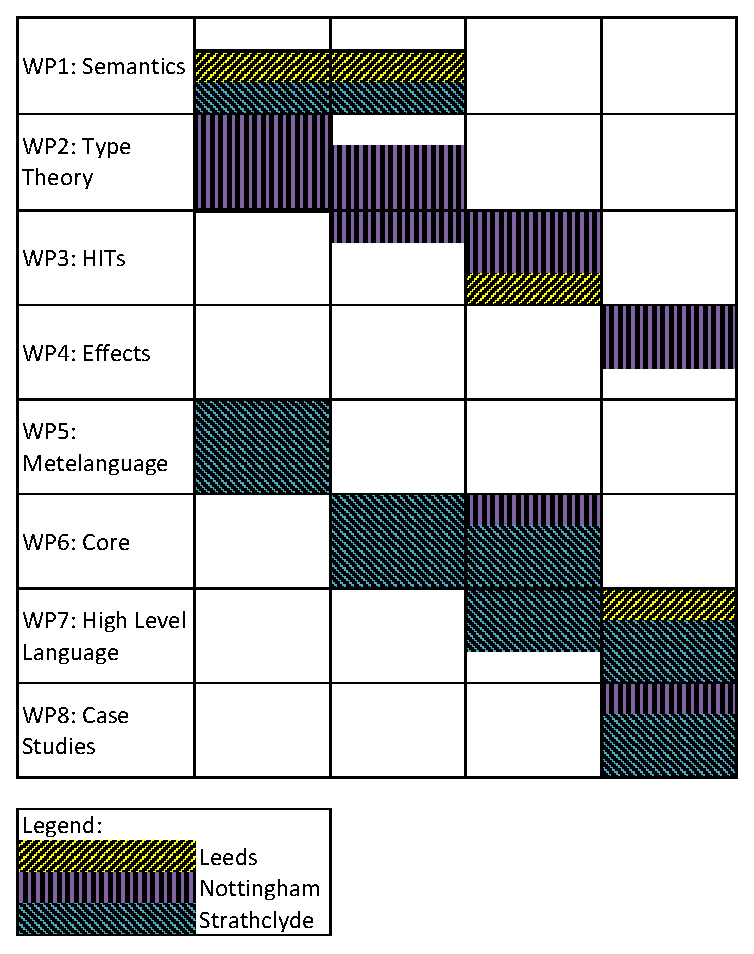
\includegraphics{Gantt.eps}
%\caption{Gantt chart depicting the order and division of work on workpackages}
%\end{figure}
%\newpage

\begin{footnotesize}
\begin{multicols}{2}
\bibliographystyle{plain}
%\bibliographystyle{abbrv}
%\bibliographystyle{plainnat}
\bibliography{proposal,alti,nicola}
\end{multicols}
\end{footnotesize}

% \begin{multicols}{2}
% \bibliographystyle{plain}
% \bibliography{proposal,alti}
% \end{multicols}{2}

\end{document}

This project will show that HoTT has just as much
potential to transform the machine checking of software correctness 
via a synthesis of theoretical, applied, and
impact-focussed research:


The cost of software failure is truly
staggering\footnote{see the sections on National Importance and
  Pathways to Impact.} and there are many successful approaches to
software verification, \eg testing, model checking etc. Formal
verification seeks mathematical guarantees of software correctness but
the complexity of modern software means that hand-written mathematical
proofs can be untrustworthy. Several decades of
research in the UK and elsewhere have culminated in systems
such as Agda, Coq, Epigram, HOL, Idris, Isabelle, NuPRL, Twelf, and
the Trellys project which offer machine-checked proofs of software
correctness. They
are having significant impact, \eg Coq won
the 2013 ACM Software and the 2013 SIGPLAN Programming Languages
awards, while HOL is used extensively by
Intel~\cite{harrison:sfm}. These systems also influence
languages with significant industrial
deployment such as Haskell, OCaml, Scala and F\#.
